\section{标量化}
\label{sec:moo-scalarization}

决策者往往能说出某种偏好：一项指标值多少钱，或者预算不能超过多少，或者希望各项都接近某个水平。有了偏好，就可以把多目标问题改写成单目标问题，再调用前面各章的方法。这样的改写称为\term{标量化}（scalarization）。

每种改写的解是不是Pareto最优点？改写的参数变化时，能到达前沿上的哪些点？要记住的一点是，标量化问题的解只代表这一次写下的偏好，不是“多目标问题的解”。

\subsection{加权和}
\label{sec:moo-weighted}

最直接的偏好是价格：给每个目标定一个单价，只看总价。这一小节研究按总价选出的方案有什么性质，以及扫遍所有价格能不能走遍前沿。

\paragraph{定义与直观}
取权重$\bm{w}$属于单纯形
\[
 \Delta_m=\Bigl\{\bm{w}\in\mathbb{R}^m:w_i\geq0,\ \sum_{i=1}^mw_i=1\Bigr\},
\]
求解
\begin{equation}
 \min_{\bm{x}\in\bm{C}}\ \sum_{i=1}^mw_if_i(\bm{x}).
 \label{eq:moo-weighted}
\end{equation}
这种做法称为\term{加权和法}（weighted-sum method）。两个目标时，把权重简写成$\bm{w}=(w,1-w)$，$w\in[0,1]$。

在目标平面上，总价相同的点组成一条法向为$\bm{w}$的直线。最小化总价，就是让这条直线从左下方平移过来，直到第一次碰到可达目标集。碰到的点就是解，这条直线称为\term{支撑线}（supporting line）。下面的讨论几乎都从这幅图景得来，见图~\ref{fig:moo-weighted-support}。

\begin{BookInlineFigure}
  \centering
  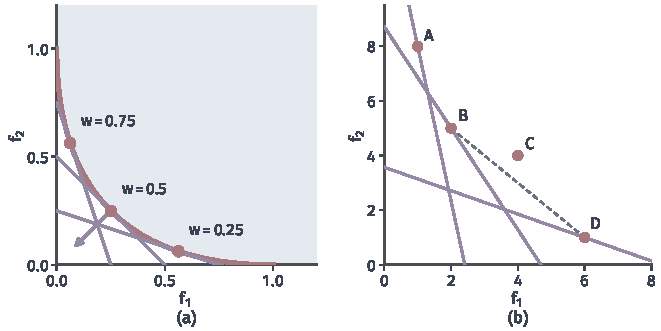
\includegraphics[width=112mm]{figures/05-optimization/07-multiple-criteria-and-nested-optimization/matplotlib/moo-weighted-support/figure.pdf}
  \caption{加权和的支撑线，紫线是最低的等总价线。(a)式~\eqref{eq:moo-iso}的前沿（红色），$w=0.25,0.5,0.75$时的切点；紫色箭头是$w=0.5$时的负法向，指向总价下降的方向。(b)式~\eqref{eq:moo-candidates}中$A,B,C,D$四点，$w=0.3,0.65,0.85$的支撑线分别经过$D,B,A$；$C$在虚线$BD$上方，任何支撑线都先碰到别的点。}
  \label{fig:moo-weighted-support}
\end{BookInlineFigure}

\paragraph{加权和的解与Pareto最优}
解的性质由权重的符号决定。权重全正时，支配者在总价上一定严格更便宜，所以解不会被支配。权重有零时，零权重目标的严格改善不计入总价，只能得到较弱的结论。

\begin{theorem}[加权和的解]
\label{thm:moo-weighted}
设$\bm{x}^\star$是问题~\eqref{eq:moo-weighted}的全局最优解。
\begin{enumerate}
 \item 若所有$w_i>0$，则$\bm{x}^\star$是Pareto最优点。
 \item 若$\bm{w}\in\Delta_m$，则$\bm{x}^\star$是弱Pareto最优点。
 \item 若$\bm{w}\in\Delta_m$，且$\bm{x}^\star$是问题~\eqref{eq:moo-weighted}的唯一全局最优解，则$\bm{x}^\star$是Pareto最优点。
\end{enumerate}
\end{theorem}

\begin{proof}
记$\phi(\bm{x})=\sum_iw_if_i(\bm{x})$。

(1)若$\bm{u}\in\bm{C}$支配$\bm{x}^\star$，则$w_if_i(\bm{u})\leq w_if_i(\bm{x}^\star)$对所有$i$成立。对$f_i(\bm{u})<f_i(\bm{x}^\star)$的那个$i$，由$w_i>0$得严格不等号。逐项相加得$\phi(\bm{u})<\phi(\bm{x}^\star)$，矛盾。

(2)若$\bm{u}\in\bm{C}$使$f_i(\bm{u})<f_i(\bm{x}^\star)$对所有$i$成立，由于$\bm{w}\in\Delta_m$，至少有一个$w_i>0$，相加仍得$\phi(\bm{u})<\phi(\bm{x}^\star)$，矛盾。

(3)若$\bm{u}\in\bm{C}$支配$\bm{x}^\star$，由$w_i\geq0$得$\phi(\bm{u})\leq\phi(\bm{x}^\star)$，所以$\bm{u}$也是全局最优解。由唯一性$\bm{u}=\bm{x}^\star$，这与“至少一项严格更小”矛盾。
\end{proof}

三条结论都只用到全局最优性，没有用到凸性。定理的第~1条马上回答了第~\ref{sec:moo-pareto}节留下的存在性问题。

\begin{theorem}[Pareto最优点的存在]
\label{thm:moo-existence}
设$\bm{C}$非空紧，各$f_i$在$\bm{C}$上连续，则Pareto解集非空。
\end{theorem}

\begin{proof}
取$w_i=1/m$。连续函数$\sum_iw_if_i$在非空紧集上取得最小值，这是第~\ref{chap:optimization}章的结论。由定理~\ref{thm:moo-weighted}的第~1条，最小点是Pareto最优点。
\end{proof}

第~\ref{sec:moo-pareto}节的反例中$\bm{C}=(0,1]$不闭，紧性不成立。

\paragraph{连续例：权重到前沿的对应}
对例~\eqref{eq:moo-iso}，由式~\eqref{eq:moo-iso-coords}，总价是
\[
 w\,s^2+(1-w)(1-s)^2+\tfrac12r^2.
\]
先取$r=0$，再对$s$求导令其为零：
\[
 2ws-2(1-w)(1-s)=0.
\]
解得$s=1-w$，也就是$\bm{x}=(w,1-w)$，对应前沿上的点
\begin{equation}
 \bigl(f_1,f_2\bigr)=\bigl((1-w)^2,\ w^2\bigr).
 \label{eq:moo-iso-weighted}
\end{equation}

前沿在该点的斜率也能算出来。由式~\eqref{eq:moo-iso-front}，$\mathrm{d}f_2/\mathrm{d}f_1=-(1-s)/s=-w/(1-w)$，正好等于等总价线的斜率。价格比决定了切点的位置，这就是图~\ref{fig:moo-weighted-support}(a)显示的情况。

例如$w=1/2$时，解是$\bm{x}=(1/2,1/2)$，目标是$(1/4,1/4)$。端点$\bm{x}=\bm{a}$只有在$w=1$时才能得到，此时权重有零，但解唯一，由定理~\ref{thm:moo-weighted}的第~3条它仍是Pareto最优点。

\paragraph{有限例：下包络}
对式~\eqref{eq:moo-candidates}，每个候选的总价是$w$的一次函数：
\[
 \begin{gathered}
  A:\ 8-7w,\quad B:\ 5-3w,\quad C:\ 4,\\
  D:\ 1+5w,\quad E:\ 6-w,\quad F:\ 1+6w.
 \end{gathered}
\]
图~\ref{fig:moo-weighted-envelope}把六条直线画在一起，每个$w$上的最小值组成红色的下包络。$w<1/2$时$D$最便宜，$1/2<w<3/4$时$B$最便宜，$w>3/4$时$A$最便宜。

\begin{BookInlineFigure}
  \centering
  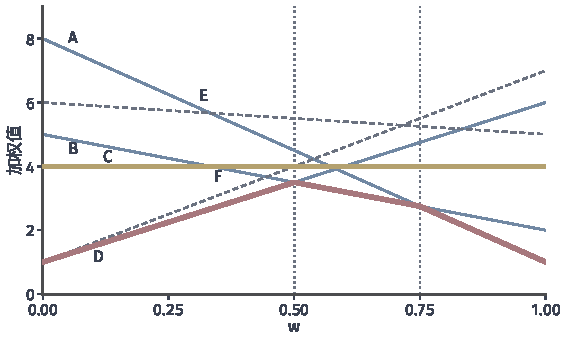
\includegraphics[width=96mm]{figures/05-optimization/07-multiple-criteria-and-nested-optimization/matplotlib/moo-weighted-envelope/figure.pdf}
  \caption{六个候选的总价随权重$w$的变化。红线是下包络，其转折点在$w=1/2$和$w=3/4$。黄线是$C$，它始终在下包络之上。虚线是被支配的$E$和$F$。}
  \label{fig:moo-weighted-envelope}
\end{BookInlineFigure}

$C$虽然是Pareto最优点，却永远选不上。要比$B$便宜，需要$4\leq5-3w$，即$w\leq1/3$；要比$D$便宜，需要$4\leq1+5w$，即$w\geq3/5$。两个要求不能同时满足。

几何上，线段$BD$在$f_1=4$处的高度是$3$，而$C$的高度是$4$，$C$位于线段上方。能被某组权重选中的Pareto点称为\term{支撑点}（supported point），$C$不是支撑点。

下包络也说明了解的跳变：$w$从小到大扫过$1/2$时，答案从$D$直接跳到$B$，两者的总价都是$3.5$；扫过$3/4$时从$B$跳到$A$，总价都是$2.75$。

零权重的情形也可以在这里看到。$w=0$时总价就是误差，$D$和$F$都等于$1$，并列最优，而$F$被$D$支配。定理~\ref{thm:moo-weighted}只保证$F$是弱Pareto最优点，这个结论不能再加强。

\paragraph{凸问题：非负权重足够覆盖}
前面的例子表明，非凸时支撑点可能不是全部。凸性保证的是，不存在$C$那样藏在凹陷里的点。

\begin{theorem}[凸问题的支撑权重]
\label{thm:moo-convex-support}
设$\bm{C}$凸，各$f_i$在$\bm{C}$上凸。若$\bar{\bm{x}}$是全局弱Pareto最优点，则存在$\bm{w}\in\Delta_m$，使$\bar{\bm{x}}$是问题~\eqref{eq:moo-weighted}的全局最优解。
\end{theorem}

证明的思路是把可达集合向右上方“加厚”，使它成为凸集，再用超平面把它与$\bar{\bm{y}}$左下方的点隔开。所用的严格分离定理在第~\ref{chap:duality}章已经证明：一点若不在闭凸集中，就存在超平面把二者严格分开。

\begin{proof}
记$\bar{\bm{y}}=\bm{f}(\bar{\bm{x}})$，记全$1$向量为$\bm{1}$。令
\[
 \bm{A}=\{\bm{f}(\bm{x})+\bm{t}:\bm{x}\in\bm{C},\ \bm{t}\geq\bm{0}\}.
\]

先说明$\bm{A}$凸。取$\bm{f}(\bm{x})+\bm{t}$与$\bm{f}(\bm{x}')+\bm{t}'$，$\gamma\in[0,1]$。由$f_i$凸，
\[
 \bm{f}(\gamma\bm{x}+(1-\gamma)\bm{x}')\leq\gamma\bm{f}(\bm{x})+(1-\gamma)\bm{f}(\bm{x}'),
\]
差额并入$\bm{t}$的凸组合，所以这两点的凸组合仍在$\bm{A}$中。于是闭包$\operatorname{cl}\bm{A}$是闭凸集。

对$\epsilon>0$，点$\bm{z}_\epsilon=\bar{\bm{y}}-\epsilon\bm{1}$不在$\operatorname{cl}\bm{A}$中。否则有$\bm{A}$中的点列趋于$\bm{z}_\epsilon$，其中某一点的每个分量都严格小于$\bar{\bm{y}}$的相应分量。这个点形如$\bm{f}(\bm{x})+\bm{t}$，于是$f_i(\bm{x})<\bar{y}_i$对所有$i$成立，与弱Pareto最优矛盾。

由严格分离定理，取单位向量$\bm{c}_\epsilon$，使对所有$\bm{x}\in\bm{C}$，$\bm{t}\geq\bm{0}$，
\[
 \langle\bm{c}_\epsilon,\bm{f}(\bm{x})+\bm{t}\rangle>\langle\bm{c}_\epsilon,\bm{z}_\epsilon\rangle.
\]
若$\bm{c}_\epsilon$有负分量，让$\bm{t}$的相应分量趋于无穷，左端趋于$-\infty$，矛盾，所以$\bm{c}_\epsilon\geq\bm{0}$。

单位球面紧，取$\epsilon\downarrow0$的子列使$\bm{c}_\epsilon\to\bm{c}$。则$\bm{c}\geq\bm{0}$，$\bm{c}\neq\bm{0}$。在上式中取$\bm{t}=\bm{0}$，令$\epsilon\downarrow0$，得到
\[
 \langle\bm{c},\bm{f}(\bm{x})\rangle\geq\langle\bm{c},\bar{\bm{y}}\rangle\quad\text{对所有}\ \bm{x}\in\bm{C}.
\]
令$\bm{w}=\bm{c}/\sum_ic_i\in\Delta_m$，上式就是$\bar{\bm{x}}$最小化$\sum_iw_if_i$。
\end{proof}

定理的结论是“存在非负权重”，不是“存在全正权重”。例~\eqref{eq:moo-iso}的端点$\bm{a}$只有权重$(1,0)$能选中，就说明全正的要求一般做不到。定理的条件也不能去掉，图~\ref{fig:moo-weighted-nonconvex}的两个例子都不满足凸性。

\paragraph{非凸前沿上的遗漏}
第三个例子是一个一元问题：$x\in[0,1]$，
\begin{equation}
 f_1(x)=x,\qquad f_2(x)=1-x^2.
 \label{eq:moo-concave}
\end{equation}
$f_1$递增，$f_2$递减，所以每个$x$都是Pareto最优点，前沿是向右上方鼓起的抛物线。加权目标是
\[
 w\,x+(1-w)(1-x^2).
\]
它是$x$的凹函数，在区间上的最小值只能在端点取到，分别是$x=0$时的$1-w$和$x=1$时的$w$。

于是$w>1/2$时解是$x=0$，$w<1/2$时解是$x=1$，$w=1/2$时两端并列。无论权重取什么，中间的方案都选不到。图~\ref{fig:moo-weighted-nonconvex}(a)中三条紫线都只能碰到两个端点。

\begin{BookInlineFigure}
  \centering
  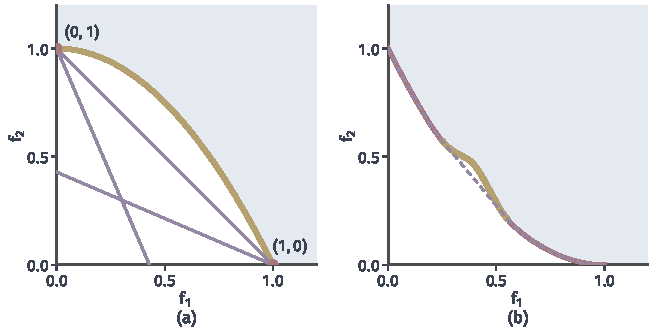
\includegraphics[width=112mm]{figures/05-optimization/07-multiple-criteria-and-nested-optimization/matplotlib/moo-weighted-nonconvex/figure.pdf}
  \caption{加权和遗漏的前沿。(a)式~\eqref{eq:moo-concave}的前沿，紫线是$w=0.3,0.5,0.7$的支撑线，都只碰到端点（红点），黄色段上的点都选不到。(b)带凹陷的前沿$f_2=(1-f_1)^2+0.1\exp(-((f_1-0.4)/0.1)^2)$，紫色虚线是它的下凸包，黄色段（$0.25<f_1<0.55$）位于凸包上方，选不到。}
  \label{fig:moo-weighted-nonconvex}
\end{BookInlineFigure}

现实中的前沿常常只有一段凹陷。图~\ref{fig:moo-weighted-nonconvex}(b)中，前沿由一个下凸的主体和一个小鼓包组成。任何方向的支撑线都不会碰到黄色段内部，紫色虚线就是它的\term{下凸包}（lower convex hull），凹陷中的点都比这条线高。从图上也可以知道，权重一旦扫过黄色段两端所对应的斜率，答案就从一端跳到另一端。

所以，“扫描权重”只能得到支撑点。对非凸问题，这可能漏掉前沿的大部分。

\subsection{阈值约束}
\label{sec:moo-threshold}

很多需求本来就不是价格，而是硬指标：预算不超过某个数，在此前提下误差尽量小。这一小节把这种需求写成约束，研究它和加权和有什么不同。

\paragraph{定义}
保留第$j$个目标作为被最小化的量，其余目标用阈值$\tau_i$限制：
\begin{equation}
 \min_{\bm{x}\in\bm{C}}\ f_j(\bm{x})
 \quad\text{s.t.}\quad f_i(\bm{x})\leq\tau_i,\ \ i\neq j.
 \label{eq:moo-threshold}
\end{equation}
这种做法称为\term{阈值约束法}（$\varepsilon$-constraint method）。这是一个普通的约束优化问题，第~\ref{chap:constrained-optimality}章的最优性条件和前一部分各章的求解方法都能直接用上。

在目标平面上，两个目标时阈值约束是一条竖线$f_1\leq\tau$，竖线左侧的部分是可行的，问题就是在其中找最低点。这条竖线不需要从外部支撑可达集合，所以能插进前沿的凹陷里。

\paragraph{解的性质}
和加权和不同，这里的结论有反方向的一半，而且不需要凸性。

\begin{theorem}[阈值约束的解]
\label{thm:moo-threshold}
固定$j$与阈值$\tau_i$，$i\neq j$。
\begin{enumerate}
 \item 问题~\eqref{eq:moo-threshold}的每个全局最优解都是弱Pareto最优点；若全局最优解唯一，它是Pareto最优点。
 \item 若$\bar{\bm{x}}$是Pareto最优点，取$\tau_i=f_i(\bar{\bm{x}})$，$i\neq j$，则$\bar{\bm{x}}$是问题~\eqref{eq:moo-threshold}的全局最优解。
 \item 设$\bm{S}$是问题~\eqref{eq:moo-threshold}的全局最优解集。若$\tilde{\bm{x}}$在$\bm{S}$上最小化$\sum_{i\neq j}f_i$，则$\tilde{\bm{x}}$是Pareto最优点。
\end{enumerate}
\end{theorem}

\begin{proof}
(1)设$\hat{\bm{x}}$是全局最优解。若$\bm{u}\in\bm{C}$的各目标都严格小于$\hat{\bm{x}}$，则$f_i(\bm{u})<f_i(\hat{\bm{x}})\leq\tau_i$，$\bm{u}$可行，而$f_j(\bm{u})<f_j(\hat{\bm{x}})$，矛盾。

若$\hat{\bm{x}}$是唯一全局最优解，设$\bm{u}$支配$\hat{\bm{x}}$。同样$\bm{u}$可行，且$f_j(\bm{u})\leq f_j(\hat{\bm{x}})$，所以$\bm{u}$也是全局最优解。由唯一性$\bm{u}=\hat{\bm{x}}$，与支配矛盾。

(2)$\bar{\bm{x}}$满足$f_i(\bar{\bm{x}})\leq\tau_i$，可行。若可行点$\bm{u}$使$f_j(\bm{u})<f_j(\bar{\bm{x}})$，再由可行性$f_i(\bm{u})\leq\tau_i=f_i(\bar{\bm{x}})$，$\bm{u}$支配$\bar{\bm{x}}$，矛盾。

(3)设$\bm{u}\in\bm{C}$支配$\tilde{\bm{x}}$。各约束下$f_i(\bm{u})\leq f_i(\tilde{\bm{x}})\leq\tau_i$，$\bm{u}$可行；又$f_j(\bm{u})\leq f_j(\tilde{\bm{x}})$，所以$\bm{u}\in\bm{S}$，且$f_j(\bm{u})=f_j(\tilde{\bm{x}})$。于是严格减小的分量在$i\neq j$中，$\sum_{i\neq j}f_i(\bm{u})<\sum_{i\neq j}f_i(\tilde{\bm{x}})$，矛盾。
\end{proof}

第~2条说的是，每个Pareto点都能被某组阈值选中，即使它不是支撑点。第~3条给出处理并列最优解的办法：先满足阈值并最小化$f_j$，再在并列的解中比较其余目标。这种分步择优也叫字典序的处理。

\paragraph{有限例与不可行}
在式~\eqref{eq:moo-candidates}上取$j=2$，以成本为预算$\tau$，求误差的最小值
\begin{equation}
 v(\tau)=\min\{f_2:f_1\leq\tau\}.
 \label{eq:moo-threshold-value}
\end{equation}
逐段比较得到：
\[
 v(\tau)=
 \begin{cases}
  \text{不可行},&\tau<1,\\
  8\ (A),&1\leq\tau<2,\\
  5\ (B),&2\leq\tau<4,\\
  4\ (C),&4\leq\tau<6,\\
  1\ (D),&\tau\geq6.
 \end{cases}
\]

这张表说明了三件事。阈值过紧时问题不可行，应当如实报告“不存在满足要求的方案”，不要输出一个违反约束的点。预算扫过$4$时选中了$C$，这个点加权和永远选不到。$\tau\geq7$时$D$与$F$并列，而$F$被$D$支配，这时按定理~\ref{thm:moo-threshold}的第~3条再比较成本，就排除了$F$。

\begin{BookInlineFigure}
  \centering
  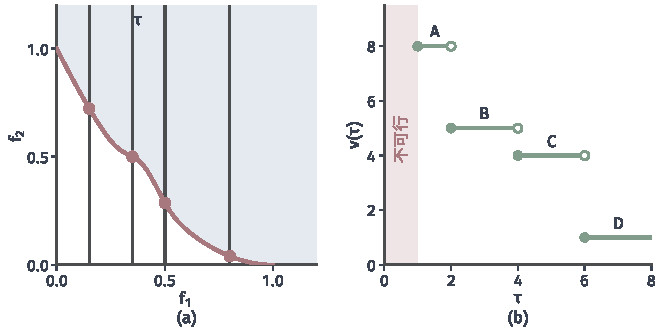
\includegraphics[width=112mm]{figures/05-optimization/07-multiple-criteria-and-nested-optimization/matplotlib/moo-threshold-scan/figure.pdf}
  \caption{阈值约束的扫描。(a)图~\ref{fig:moo-weighted-nonconvex}(b)的前沿，深灰竖线是四个阈值，红点是相应的解，其中两个点在加权和选不到的凹陷段内。(b)有限例的$v(\tau)$，实心点属于该段，空心点不属于；粉色区域不可行，字母是选中的方案。}
  \label{fig:moo-threshold-scan}
\end{BookInlineFigure}

图~\ref{fig:moo-threshold-scan}(a)显示，阈值从左向右扫过时，解沿整条前沿移动。代价是每次都要解一个带约束的问题，这比加权和难：加权和只是一个无约束问题，这里多了一个可能起作用的约束。

\paragraph{阈值与价格的联系}
阈值$\tau$和价格$w$看起来是两种语言，通过乘子可以把它们联系起来。把例~\eqref{eq:moo-iso}写成$j=2$的阈值问题，
\[
 \min\ f_2(\bm{x})\quad\text{s.t.}\quad f_1(\bm{x})\leq\tau,
\]
约束起作用时，KKT驻定条件（第~\ref{chap:constrained-optimality}章）要求
\begin{equation}
 \nabla f_2(\bm{x})+\lambda\nabla f_1(\bm{x})=\bm{0},\qquad\lambda\geq0.
 \label{eq:moo-threshold-kkt}
\end{equation}

式~\eqref{eq:moo-threshold-kkt}除以$1+\lambda$，就是权重$\bm{w}=(\lambda,1)/(1+\lambda)$的加权和的驻定条件。乘子$\lambda$就是目标$f_1$相对于$f_2$的价格。

具体计算。在解的线段上$f_1=s^2=\tau$，所以$s=\sqrt\tau$，且$r=0$。式~\eqref{eq:moo-threshold-kkt}沿线段方向的分量给出$(s-1)+\lambda s=0$，于是
\begin{equation}
 \lambda(\tau)=\frac{1-\sqrt\tau}{\sqrt\tau},\qquad 0<\tau\leq1.
 \label{eq:moo-iso-lambda}
\end{equation}

例如$\tau=1/4$时，$s=1/2$，$\lambda=1$，权重正是$(1/2,1/2)$，解与式~\eqref{eq:moo-iso-weighted}中$w=1/2$的解相同。

式~\eqref{eq:moo-iso-lambda}也描述了$\tau$增大时价格怎样变化。由式~\eqref{eq:moo-iso-front}，最优值$v(\tau)=(1-\sqrt\tau)^2$，求导得
\[
 v'(\tau)=-\frac{1-\sqrt\tau}{\sqrt\tau}=-\lambda(\tau).
\]
放宽一单位阈值，最优值下降$\lambda$，这与第~\ref{chap:parametric-sensitivity}章乘子是影子价格的结论一致。图~\ref{fig:moo-threshold-price}画出了这一点。$\tau$接近$0$时$\lambda$趋于无穷，$\tau\geq1$时约束不再起作用，$\lambda=0$，解停在$\bm{b}$。

\begin{BookInlineFigure}
  \centering
  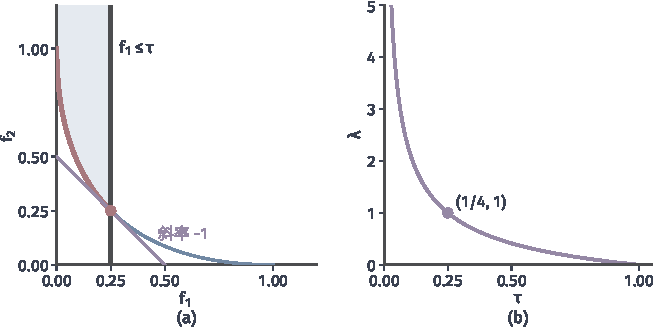
\includegraphics[width=112mm]{figures/05-optimization/07-multiple-criteria-and-nested-optimization/matplotlib/moo-threshold-price/figure.pdf}
  \caption{阈值与价格，例~\eqref{eq:moo-iso}。(a)深灰竖线是阈值$f_1\leq1/4$，可行部分为左侧浅蓝区域，红色段是可行的前沿，红点是解；紫线是前沿在该点的切线，斜率$-\lambda=-1$。(b)乘子随阈值的变化，式~\eqref{eq:moo-iso-lambda}。}
  \label{fig:moo-threshold-price}
\end{BookInlineFigure}

这种对应只在问题有相应结构时才是一一对应。非凸时，凹陷中的解仍满足式~\eqref{eq:moo-threshold-kkt}，但它只是相应加权和的驻定点，不是最小点。阈值问题的解能到达加权和到不了的地方，正是因为这里的约束替代了全局的比较。

\paragraph{并列最优解}
前沿出现水平段时，阈值问题的解不唯一。图~\ref{fig:moo-threshold-tie}中，阈值$\tau$落在底部水平边的范围内，$\bm{z}'$和$\bm{z}$的$f_2$都等于最小值，黄色线段上的点都是最优解。$\bm{z}$被$\bm{z}'$支配。

\begin{BookInlineFigure}
  \centering
  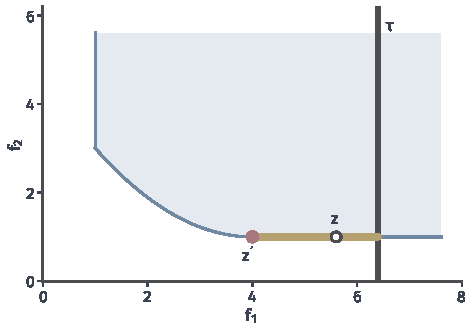
\includegraphics[width=80mm]{figures/05-optimization/07-multiple-criteria-and-nested-optimization/matplotlib/moo-threshold-tie/figure.pdf}
  \caption{阈值约束的并列最优解。深灰竖线是阈值，黄色线段是$\min\{f_2:f_1\leq\tau\}$的全部解的目标值。空心点$\bm{z}$是弱Pareto最优点，红点$\bm{z}'$是在并列解中进一步最小化$f_1$后得到的Pareto最优点。}
  \label{fig:moo-threshold-tie}
\end{BookInlineFigure}

求解器一般只返回并列解中的某一个，不一定是$\bm{z}'$。所以，只要阈值问题的解不能确认唯一，就要做第二阶段的择优，否则报告的只是一个弱Pareto最优点。

\subsection{参考点方法}
\label{sec:moo-reference}

有时决策者说的既不是价格，也不是预算，而是希望各项指标都接近某个水平。这一小节把这种需求写成到参考点的最大偏差，它能选中加权和选不到的点，又不必增加约束。

\paragraph{定义}
设各目标在$\bm{C}$上有有限下界，取\term{参考点}（reference point）$\bm{z}$，使$z_i<\inf_{\bm{C}}f_i$对所有$i$成立。再取权重$w_i>0$，最小化带权的最大偏差：
\begin{equation}
 \min_{\bm{x}\in\bm{C}}\ \max_{1\leq i\leq m}\ w_i\bigl(f_i(\bm{x})-z_i\bigr).
 \label{eq:moo-chebyshev}
\end{equation}
这种做法称为\term{加权Chebyshev标量化}（weighted Chebyshev scalarization）。

式~\eqref{eq:moo-chebyshev}的直观含义是，目标被缩放后，看离参考点最远的一项。下水平集是以$\bm{z}$为左下角的长方形，边长比由权重决定。随着水平增大，长方形的右上角沿着从$\bm{z}$出发、方向为$(1/w_1,\ldots,1/w_m)$的射线向外移动。长方形第一次碰到可达集合时的水平，就是最优值。

长方形的右上角尖尖地探出去，而加权和的直线是平的。平的直线碰不到凹陷，尖的角能探进去，见图~\ref{fig:moo-chebyshev-level}。

\begin{BookInlineFigure}
  \centering
  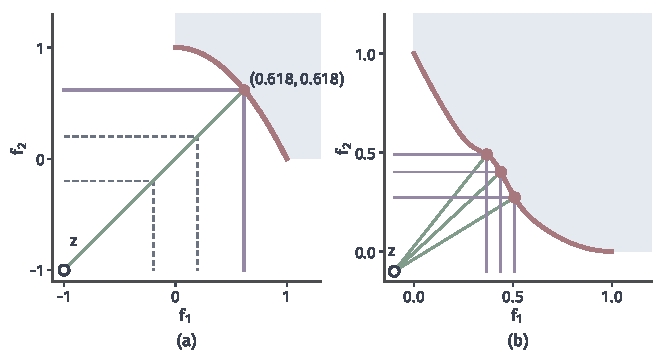
\includegraphics[width=112mm]{figures/05-optimization/07-multiple-criteria-and-nested-optimization/matplotlib/moo-chebyshev-level/figure.pdf}
  \caption{加权Chebyshev的水平集，空心点是参考点$\bm{z}$，绿线是沿$(1/w_1,1/w_2)$的射线。(a)式~\eqref{eq:moo-concave}的前沿，$\bm{z}=(-1,-1)$，$\bm{w}=(1/2,1/2)$；灰色虚线是较低水平的长方形边界，紫线是最优水平，角落碰到$(0.618,0.618)$。(b)图~\ref{fig:moo-weighted-nonconvex}(b)的前沿，$\bm{z}=(-0.1,-0.1)$，三组权重的解都在凹陷段内，紫线是相应的最优长方形边界。}
  \label{fig:moo-chebyshev-level}
\end{BookInlineFigure}

\paragraph{解的性质}
先看式~\eqref{eq:moo-chebyshev}的解是什么点，再看能选到哪些点。

\begin{theorem}[加权Chebyshev的解]
\label{thm:moo-chebyshev}
设$\bm{z}$严格低于各目标的下确界。
\begin{enumerate}
 \item 对任意$w_i>0$，问题~\eqref{eq:moo-chebyshev}的全局最优解都是弱Pareto最优点。
 \item 若$\bar{\bm{x}}$是弱Pareto最优点，取
 \begin{equation}
  w_i=\frac{1}{f_i(\bar{\bm{x}})-z_i},
  \label{eq:moo-chebyshev-weight}
 \end{equation}
 则$\bar{\bm{x}}$是问题~\eqref{eq:moo-chebyshev}的全局最优解。
 \item 设$\bm{S}$是问题~\eqref{eq:moo-chebyshev}的全局最优解集。若$\tilde{\bm{x}}$在$\bm{S}$上最小化$\sum_if_i$，则$\tilde{\bm{x}}$是Pareto最优点。
\end{enumerate}
\end{theorem}

\begin{proof}
记$\psi(\bm{x})=\max_iw_i(f_i(\bm{x})-z_i)$。

(1)设$\bm{x}^\star$是全局最优解。若$\bm{u}$的各目标都严格小于$\bm{x}^\star$，由$w_i>0$，对所有$i$有
\[
 w_i(f_i(\bm{u})-z_i)<w_i(f_i(\bm{x}^\star)-z_i)\leq\psi(\bm{x}^\star).
\]
有限个严格不等式取最大仍严格，$\psi(\bm{u})<\psi(\bm{x}^\star)$，矛盾。

(2)由$z_i<\inf f_i$，式~\eqref{eq:moo-chebyshev-weight}中分母为正，$w_i>0$，并且
\[
 w_i\bigl(f_i(\bar{\bm{x}})-z_i\bigr)=1\quad\text{对所有}\ i,
\]
所以$\psi(\bar{\bm{x}})=1$。若有$\bm{u}$使$\psi(\bm{u})<1$，则$w_i(f_i(\bm{u})-z_i)<1$对所有$i$成立，代入$w_i$的定义得$f_i(\bm{u})<f_i(\bar{\bm{x}})$对所有$i$成立，与弱Pareto最优矛盾。

(3)设$\bm{u}$支配$\tilde{\bm{x}}$。各项$f_i(\bm{u})\leq f_i(\tilde{\bm{x}})$，由$w_i>0$得$\psi(\bm{u})\leq\psi(\tilde{\bm{x}})$，所以$\bm{u}\in\bm{S}$。又有一项严格减小，$\sum_if_i(\bm{u})<\sum_if_i(\tilde{\bm{x}})$，矛盾。
\end{proof}

$\bm{z}$严格低于下确界的条件保证了第~2条的权重有限且为正。第~2条不需要凸性，这也是这种标量化比加权和强的地方：调整权重可以选中每一个弱Pareto最优点，当然也包括每一个Pareto最优点。

\paragraph{算一个连续的例子}
对式~\eqref{eq:moo-concave}取$\bm{z}=(-1,-1)$，它低于两个目标的下确界$0$。取$\bm{w}=(1/2,1/2)$，目标是
\[
 \psi(x)=\frac12\max\bigl\{x+1,\ 2-x^2\bigr\}.
\]
$x+1$递增，$2-x^2$递减，最大值的最小点在两者相等处：
\[
 x+1=2-x^2,\quad\text{即}\quad x^2+x-1=0.
\]
解得$x=(\sqrt5-1)/2\approx0.618$，目标向量也是$(0.618,0.618)$，这是加权和选不到的中间点。

\paragraph{有限例：并列最优仍会发生}
在式~\eqref{eq:moo-candidates}上取$\bm{z}=(0,0)$，它严格低于下确界$(1,1)$。取$\bm{w}=(1/2,1/2)$，各候选的$\psi$值为
\[
 A:\ 4,\quad B:\ 2.5,\quad C:\ 2,\quad D:\ 3,\quad E:\ 3,\quad F:\ 3.5.
\]
最小的是$C$，这正是加权和选不到的方案，见图~\ref{fig:moo-chebyshev-finite}(a)。

再取$\bm{w}=(0.1,0.9)$，各候选的$\psi$值为
\[
 A:\ 7.2,\quad B:\ 4.5,\quad C:\ 3.6,\quad D:\ 0.9,\quad E:\ 5.4,\quad F:\ 0.9.
\]
$D$与$F$并列最小。此时第二个目标的偏差决定了最大值，第一个目标的差别被$\max$吞掉了，$F$虽然被$D$支配，却同样最优，见图~\ref{fig:moo-chebyshev-finite}(b)。按定理~\ref{thm:moo-chebyshev}的第~3条再比较$\sum_if_i$，$D$的和是$7$，$F$的和是$8$，排除了$F$。

\begin{BookInlineFigure}
  \centering
  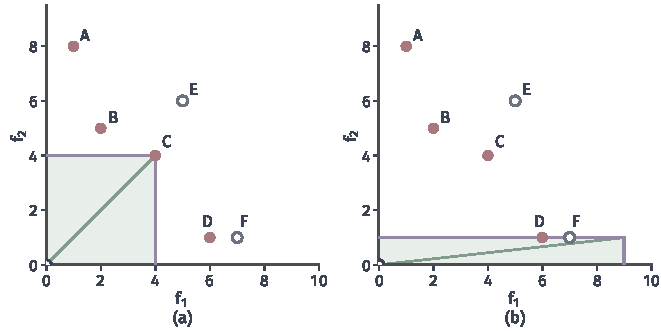
\includegraphics[width=112mm]{figures/05-optimization/07-multiple-criteria-and-nested-optimization/matplotlib/moo-chebyshev-finite/figure.pdf}
  \caption{有限候选上的加权Chebyshev，参考点$\bm{z}=(0,0)$（空心点在原点）。绿色长方形是最优水平的下水平集，紫线是其右上边界。(a)$\bm{w}=(1/2,1/2)$，长方形的角落碰到$C$。(b)$\bm{w}=(0.1,0.9)$，长方形的上边同时碰到$D$和$F$，$F$是并列的弱Pareto最优点。}
  \label{fig:moo-chebyshev-finite}
\end{BookInlineFigure}

\paragraph{三种写法的比较}
表~\ref{tab:moo-scalarization}汇总了三种标量化。没有哪一种处处占优。加权和最容易求解，但只能到达支撑点；阈值约束和加权Chebyshev能到达每个Pareto点，代价是多了约束或非光滑的$\max$。后者可以用第~\ref{chap:quadratic-conic-programming}章一类的上图改写来处理：引入变量$t$，在约束$w_i(f_i(\bm{x})-z_i)\leq t$下最小化$t$。

\begin{BookInlineTable}
  \centering
  \caption{三种标量化的比较。“解的保证”指全局最优解的性质。}
  \label{tab:moo-scalarization}
  \begin{tabular}{@{}llll@{}}
    \toprule
    方法 & 解的保证 & 可达的点 & 并列情形\\
    \midrule
    加权和 & 全正权：Pareto & 支撑点 & 权重有零时\\
    阈值约束 & 弱Pareto & 全部Pareto点 & 水平段上\\
    加权Chebyshev & 弱Pareto & 全部弱Pareto点 & 水平段或竖直段\\
    \bottomrule
  \end{tabular}
\end{BookInlineTable}

这些结论的更多变形可以查阅凸优化专著中多准则优化一节\scite{math-boyd2004convex}。无论用哪一种，所得的都只是一次偏好下的解。要给决策者看一组候选，还需要第~\ref{sec:moo-front-computation}节的组织方式。
